\chapter{Linear Analysis}
\label{chp:AnalNumMethod}
In this chapter a linear analysis is used to study the convergence and dispersion properties of the numerical methods. 

An important property of a numerical method is convergence. Convergence guarantees that as the spatial and temporal resolution of a numerical method is increased, then the numerical solution approaches the solution of the partial differential equations it approximates. 

For linear partial differential equations the Lax-equivalence theorem states that a numerical method is convergent if and only if it is stable and consistent \cite{Lax-Richtmyer-1956-267}. A numerical scheme is consistent if the error introduced by the numerical method over a time step approaches zero as the spatial and temporal resolution increases. A numerical method is stable if the errors from previous time steps are not amplified over subsequent time steps.

Another important attribute of a numerical method modelling dispersive wave equations, such as the Serre equations is its dispersion properties. The dispersion relation of a system determines the phase and group velocity of travelling waves in that system. The Serre equations possess a dispersion relation that well approximates the dispersion relation given by linear theory for water waves \cite{Barthelemy-2004-315}. Therefore, how well the dispersion relation of a numerical method approximates the dispersion relation of the Serre equations is of particular interest.

We analysed the convergence and dispersion properties of the whole numerical method applied to the solution of the linearised Serre equations with a horizontal bed. The whole scheme is considered with the spatial and temporal approximations analysed simultaneously. The effect of variations in the bed and non-linear terms are important when studying the convergence properties of our methods for solving the full Serre equations. However, these effects greatly increase the complexity of the convergence analysis. We therefore, estimate the convergence properties of the non-linear Serre equations with varying bathymetry by investigating the linearised Serre equations with a horizontal bed. 

In general, we would expect that a numerical method that has poor convergence properties for the linearised Serre equations with a horizontal bed will also have poor convergence properties when the bed and non-linear terms are included. 

The dispersion properties of the Serre equations are derived from the linearised Serre equations with a horizontal bed \cite{Zoppou-etal-2017}. Because the dispersion analysis includes the spatial and temporal approximations simultaneously the presented analysis of dispersion properties of the numerical method is a complete analysis extending the work of \citet{Filippini-etal-2016-381}.

The linear analyses of convergence and dispersion properties for the finite volume based methods rely on establishing a relationship of the form
\begin{equation}
\label{eqn:linearanalaim}
\begin{bmatrix}
\overline{h} \\\overline{G} 
\end{bmatrix}^{n+1}_j = \matr{E} \begin{bmatrix}
\overline{h} \\\overline{G}
\end{bmatrix}^{n}_j
\end{equation}
where $\matr{E}$ is the $2 \times 2$ evolution matrix relating the cell average conserved quantities $h$ and $G$ at time level $t^n$ with the cell average conserved quantities at time level $t^{n+1}$, which is independent of $n$ and $j$. The evolution matrix $\matr{E}$ is obtained in the analyses by propagating Fourier modes through the numerical scheme. By analysing the properties of $\matr{E}$ and comparing it with the exact evolution matrix we can determine the convergence and dispersion properties of its associated numerical method.
 
We derive $\matr{E}$ in \eqref{eqn:linearanalaim} for $\text{FEVM}_2$ and perform the convergence and dispersion analysis. We then present the results of the analyses for the finite difference volume methods $\text{FDVM}_1$, $\text{FDVM}_2$ and $\text{FDVM}_3$ described by \citet{Zoppou-etal-2017} and the finite difference methods $\mathcal{D}$ and $\mathcal{W}$ described by \citet{Pitt-2018-61}. These results extend those published by \citet{Zoppou-etal-2017} by including more methods, analysing the convergence properties and allowing non-zero background mean velocities.
 
\section{Linearised Serre Equations}
The Serre equations with a horizontal bed \eqref{eqn:FullSerreNonConHorizbed} are linearised by considering waves as small perturbations $\delta\times\eta(x,t)$ and $\delta \times\mu(x,t)$ on a flow with a mean height $H$ and a mean velocity $U$ respectively, where $\delta \ll 1$. So we have
\begin{subequations}
	\label{eq:pertubation}
\begin{align}
h(x,t) &= H + \delta \eta(x,t) + \mathcal{O}\left(\delta^2 \right), \\
u(x,t) &= U + \delta \mu(x,t) + \mathcal{O}\left(\delta^2 \right).
\end{align}
\end{subequations} These waves are relatively small so terms of order $\delta^2$ are negligible. We substitute \eqref{eq:pertubation} into the Serre equations and neglect terms of order $\delta^2$ to obtain

\begin{subequations}
	\label{eqn:LinAll}
	\begin{align}
		\label{eqn:LinCont}
		&\frac{\partial  \left(\delta\eta \right)}{\partial  t} + H\frac{\partial  \left(\delta\mu \right)}{\partial  x} + U\frac{\partial  \left(\delta\eta \right)}{\partial  x}  = 0, \\
	\label{eqn:LineMome}
	&H\frac{\partial  \left(\delta\mu \right)}{\partial  t} + gH\frac{\partial  \left(\delta\eta \right)}{\partial  x} + UH\frac{\partial  \left(\delta\mu \right)}{\partial  x} - \frac{H^3}{3}\left(U\frac{\partial^3  \left(\delta\mu \right)}{\partial  x^3} + \frac{\partial^3  \left(\delta\mu \right)}{\partial  x^2 \partial  t}  \right)  = 0
	\end{align}	
and for $G$
\begin{equation}
	G = UH + U \delta \eta + H \delta \mu -\frac{H^3}{3} \frac{\partial^2 \left(\delta\mu \right)}{\partial x^2}.
	\label{eqn:LinConSerreGu0}
\end{equation}	
	\label{eqn:LinConSerre}
\end{subequations}
Absorbing the $\delta$ factor into the corresponding $\eta$ and $\mu$ terms and rewriting these equations in conservation law form for $\eta$ and $G$ we obtain
\begin{subequations}
	\begin{align}
	\label{eqn:LinContG}
	&\frac{\partial  \eta}{\partial  t} +\frac{\partial}{\partial  x} \left(H\mu + U \eta\right) = 0, \\
	\label{eqn:LineMomeG}
	&\frac{\partial  G}{\partial  t} + \frac{\partial}{\partial  x}\left(UG + UH\mu + gH \eta\right) = 0
	\end{align}
	where
	\begin{equation}
	G = UH + U \eta + H \mu -\frac{H^3}{3} \frac{\partial^2 \mu }{\partial x^2}.
	\label{eqn:LinConSerreG}
	\end{equation}
	\label{eqn:LinSerreG}	
\end{subequations}

\section{Evolution Matrix}
To derive the evolution matrix, $\matr{E}$ we study the behaviour of \eqref{eqn:LinSerreG} when $\eta$ and $\mu$ are Fourier modes. A Fourier mode $q(x,t)$ is
\begin{equation}
q(x,t) = q(0,0) e^{i\left(\omega^\pm t + kx\right)}
\label{eqn:FourierNode}
\end{equation}
where $k$ is the wavenumber, $\omega^\pm$ is the frequency \eqref{eqn:DispersionRelation} and $i$ is the imaginary number. The Fourier modes are the eigenfunctions of these linearised Serre equations \eqref{eqn:LinSerreG}. Since the eigenfunctions form a basis of the solution space, their dispersion and convergence properties are inherited by all solutions of \eqref{eqn:LinSerreG}. Therefore, it is sufficient to study only the convergence and dispersion properties for Fourier mode solutions captured by the evolution matrix $\matr{E}$. 

A consequence of a quantity $q$ being a Fourier mode represented on a uniform temporal and spatial grid is that for any real numbers $m$ and $l$ we have
\begin{equation}
q^{n + m}_{j + l} = q^n_j e^{ i \left(m \omega^\pm \Delta t + l k \Delta x\right)}.
\label{eqn:fourierfactor}
\end{equation}
Because $\eta$ and $\mu$ are Fourier modes then so is $G$. Furthermore, the cell averages of these quantities $\overline{\eta}$, $\overline{\mu}$ and $\overline{G}$ are Fourier modes as well.

For Fourier modes the operators $\mathcal{R}^+_{j-1/2}$, $\mathcal{R}_{j}$, $\mathcal{R}^-_{j+1/2}$, $\mathcal{G}$, $\mathcal{F}_{j-1/2}$ and $\mathcal{F}_{j+1/2}$ from Chapter \ref{chp:HFVMMethod} will only vary with $H$, $U$, $k$, $\omega^\pm$, $\Delta x$ and $\Delta t$ and hence are independent of $j$ and $n$. By combining these operators the evolution matrix $\matr{E}$ can be derived for $\text{FEVM}_2$ for the linearised Serre equations with a horizontal bed. Since all the constituent operators of $\matr{E}$ are independent of $j$ and $n$ then $\matr{E}$ will also be independent of $j$ and $n$, as desired. We will now derive expressions for all these operators, following the structure of the method laid out in Section \ref{sec:StructOverview}. Since the linearised Serre equations with a horizontal bed have no source terms step (iv), which approximates the source terms is not necessary.   

\subsection{Reconstruction}
Given the cell averages $\overline{\vecn{\eta}}$ and $\overline{\vecn{G}}$ at $t^n$, the first step of our numerical method is to reconstruct $\eta$ and $G$ inside the $j^{th}$ cell at $x_{j-1/2}$, $x_j$ and $x_{j+1/2}$ using $\mathcal{R}^+_{j-1/2}$, $\mathcal{R}_{j}$ and $\mathcal{R}^-_{j+1/2}$ from \eqref{eqn:ReconforhwG}. Since $\eta$ and $G$ are Fourier modes and therefore smooth we do not require non-linear limiters to ensure our scheme is TVD and so we use the slope $d_j = \left({-\overline{q}_{j-1} +\overline{q}_{j+1}}\right)/ \left({2\Delta x} \right)$ in the reconstruction. Applying \eqref{eqn:fourierfactor} to the reconstructions \eqref{eqn:ReconforhwG} with the centred slope approximation we obtain 

\begin{subequations}
	\label{eqn:RpmfactorFDVM}
	\begin{align}
	q^+_{j-\frac{1}{2}} &= \overline{q}_j - \frac{- \overline{q}_{j} e^{-ik\Delta x} + \overline{q}_{j} e^{ik\Delta x}}{4} = \left(1  - \frac{i\sin\left(k\Delta x\right)}{2} \right)\overline{q}_{j} = \mathcal{R}^+_{j-1/2}\overline{q}_{j}, \\
	q_j &= \overline{q}_j = \mathcal{R}_{j} \overline{q}_j,\\
	q^-_{j+\frac{1}{2}} &=\overline{q}_j + \frac{- \overline{q}_{j} e^{-ik\Delta x} + \overline{q}_{j} e^{ik\Delta x}}{4} = \left(1  + \frac{i\sin\left(k\Delta x\right)}{2} \right)\overline{q}_{j} =\mathcal{R}^-_{j+1/2} \overline{q}_{j}.
	\end{align}
Note that these reconstructions operators $\mathcal{R}^+_{j-1/2}$, $\mathcal{R}_{j}$ and $\mathcal{R}^-_{j+1/2}$ are independent of $j$. Furthermore, from \eqref{eqn:fourierfactor} we have that reconstructions of $\eta$ and $G$ at other locations are $\mathcal{R}^+_{j-1/2}$, $\mathcal{R}_{j}$ and $\mathcal{R}^-_{j+1/2}$ multiplied by a shift factor. In particular, we have that the reconstruction operator $\mathcal{R}^+_{j+1/2}$ for $q^+_{j+\frac{1}{2}} $ is given by
\begin{equation}
	q^+_{j+\frac{1}{2}} = e^{ik\Delta x} q^+_{j-\frac{1}{2}} = e^{ik\Delta x} \mathcal{R}^+_{j-1/2}\overline{q}_{j} = \mathcal{R}^+_{j+1/2}\overline{q}_{j}.
\end{equation}
\end{subequations}  


\subsection{Fluid Velocity}
To calculate the velocity perturbation $\mu_{j+1/2}$ we use a second-order FEM. We begin with the weak formulation of \eqref{eqn:LinConSerreG}, obtained by multiplying \eqref{eqn:LinConSerreG} by a test function $v$ and integrating over the spatial domain $\Omega$
\begin{equation*}
\int_{\Omega}G v \; dx = UH\int_{\Omega} v \; dx + U \int_{\Omega} \eta v \; dx +   H\int_{\Omega} \mu v \; dx  + \frac{H^3}{3} \int_{\Omega} \frac{\partial \mu}{\partial x } \frac{\partial v}{\partial x }\; dx.
\end{equation*}
The FEM then proceeds for \eqref{eqn:LinConSerreG} as in Chapter \ref{chp:HFVMMethod} for the non-linear Serre equation. So that $G$ has the basis functions $\psi^+_{j - 1/2}$ and $\psi^-_{j + 1/2}$ \eqref{eqn:App1:PsiDef}, which means our approximation to $G$ is linear inside a cell with discontinuous jumps at the cell edges. For $v$ and $\mu$ the basis functions $\phi_{j-1/2}$, $\phi_{j}$ and $\phi_{j+1/2}$ \eqref{eqn:App1:PhiDef} are used so that $v$ and our approximation to $\mu$ are quadratic polynomials inside a cell and are continuous across the cell edges.

Given the detailed description of the method in Chapter \ref{chp:HFVMMethod}, we will just present the element wise matrix $\matr{A}_j$ and vector $\vecn{g}_j$ for the finite element approximation to \eqref{eqn:LinSerreG} 
\begin{align*}
\matr{A}_j &= H \frac{\Delta x}{30 } \begin{bmatrix} \TM 4 &2 &-1 \\2 &16 &2  \\-1 &2 &4 \BM \end{bmatrix} +  \frac{H^3 }{3} \frac{1 }{3\Delta x}\begin{bmatrix} \TM 7 &-8 &1  \\-8 &16 &-8  \\1 &-8 &7 \BM \end{bmatrix}, \\
\vecn{g}_j &=  \frac{\Delta x}{6} \left(\begin{bmatrix} \TM G^+_{j -1/2} \\2 G^+_{j -1/2}+2 G^-_{j +1/2} \\ G^-_{j +1/2} \BM \end{bmatrix} - UH\begin{bmatrix} \TM 1 \\4 \\ 1  \BM\end{bmatrix} - U\begin{bmatrix} \TM \eta^+_{j -1/2} \\2 \eta^+_{j -1/2}+2 \eta^-_{j +1/2} \\ \eta^-_{j +1/2} \end{bmatrix} \BM \right).
\end{align*}
To calculate the intercell flux we require $\mu$ at $x_{j+1/2}$. From the element wise matrices and vectors for the $j^{th}$ and $\left(j+1\right)^{th}$ cells the equation that relates all the quantities at $x_{j+1/2}$ is
\begin{multline*}
\frac{\Delta x}{6} \left(G^-_{j +1/2} + G^+_{j +1/2} \right)= \\
2UH \frac{\Delta x}{6}   + U\frac{\Delta x}{6} \left(\eta^-_{j +1/2} + \eta^+_{j +1/2} \right) \\ +   \Bigg(H\frac{\Delta x}{30} \Bigg[ -\mu_{j-1/2} +  2\mu_{j} + 8\mu_{j+1/2}  +  2 \mu_{j+1}  - \mu_{j+3/2}\Bigg]   \\ + \frac{H^3 }{3}\frac{1 }{3\Delta x} \Bigg[  \mu_{j-1/2} -8\mu_{j} + 14 \mu_{j+1/2} -8\mu_{j+1} + \mu_{j+3/2}  \Bigg]    \Bigg).
\end{multline*}
Using \eqref{eqn:RpmfactorFDVM} and \eqref{eqn:fourierfactor}, we obtain
\begin{multline*}
\frac{\Delta x}{6} \left(\mathcal{R}^-_{j +1/2} + \mathcal{R}^+_{j +1/2} \right) \overline{G}_j =  \\
2UH\frac{\Delta x}{6}   + U\frac{\Delta x}{6} \left(\mathcal{R}^-_{j +1/2} + \mathcal{R}^+_{j +1/2} \right) \overline{\eta}_j\\ +   \Bigg(H\frac{\Delta x}{30} \Bigg[ -e^{-ik\Delta x } +  2 e^{-ik\frac{\Delta x}{2}}  + 8 + 2 e^{ik\frac{\Delta x}{2}} - e^{ik{\Delta x}}  \Bigg]   \\ + \frac{H^3 }{3}\frac{1 }{3\Delta x} \Bigg[  e^{-ik{\Delta x}} -8e^{-ik\frac{\Delta x}{2}} + 14  - 8 e^{ik\frac{\Delta x}{2}} + e^{ik{\Delta x}}  \Bigg]    \Bigg) \mu_{j+1/2}. 
\end{multline*}
Rearranging the equation we have that
\begin{align}
\label{eqn:2ndFEMutoG}
\mu_{j+1/2} =  \mathcal{G}^{\eta} \overline{\eta}_{j} + \mathcal{G}^G \overline{G}_{j} + \mathcal{G}^c 
\end{align}
where
\begin{align*}
\mathcal{G}^\eta &=  -U\mathcal{G}^G, \\ \\
\mathcal{G}^G &= \dfrac{\Delta x}{6\mathcal{G}_D } \left(\mathcal{R}^-_{j +1/2} + \mathcal{R}^+_{j +1/2} \right), \\ \\
\mathcal{G}^c &=  -2UH \dfrac{\Delta x}{6\mathcal{G}_D }
\end{align*}
and the common divisor $\mathcal{G}_D$ is
\begin{multline*}
\mathcal{G}_D = H\frac{\Delta x}{30} \left(4\cos\left(\frac{k \Delta x}{2}\right) - 2\cos\left({k \Delta x}\right) + 8\right) \\ + \frac{H^3 }{3}\frac{1}{3\Delta x}\left(-16\cos\left(\frac{k\Delta x}{2}\right) + 2 \cos\left(k \Delta x\right) + 14\right).
\end{multline*}
So that the factors $\mathcal{G}^\eta$, $\mathcal{G}^G$ $\mathcal{G}^c$ do not depend on $n$ or $j$ as desired.

\subsection{Flux Across the Cell Interfaces}
%LIST THE FACTORS FIRST!!!!
The average intercell flux $F_{j+1/2}$ is approximated using \eqref{eqn:HLL_flux}. For the linearised Serre equations we have the wave speed bounds \eqref{eqn:WaveVelocitiesBound}, so that
\begin{align}
a^-_{j+ 1/2} = \min \left\lbrace 0,  U - \sqrt{g H} \right \rbrace&, &a^+_{j+ 1/2} =  \max \left\lbrace 0, U + \sqrt{g H} \right \rbrace .
\label{eqn:wavespeedboundslinSerre}
\end{align}

This method has three different approximations to $F_{j+1/2}$ depending on the Froude number $Fr = {U}/{\sqrt{gH}}$; (i)
supercritical flow to the left where $Fr < -1$, (ii) critical and subcritical flow in both directions where $-1 \le Fr \le 1$ and (iii) supercritical flow to the right where $Fr > 1$. We will derive the flux operators for each of these cases separately.

\subsubsection{Left Supercritical Flow $Fr < -1$:}
For left supercritical flow; $Fr < -1$ and therefore $U + \sqrt{g H} < 0$ so we have from \eqref{eqn:wavespeedboundslinSerre} that $a^-_{j+ 1/2} = U - \sqrt{g H}$ and $a^+_{j+ 1/2} =  0$. For these values the flux approximation reduces to 
\begin{equation}
F_{j+\frac{1}{2}} = f\left(q^+_{j+\frac{1}{2}}\right)
\label{eqn:fluxleftsupercrit}
\end{equation}
for a generic quantity $q$.

Substituting the flux function from the continuity equation \eqref{eqn:LinContG} into the flux approximation we obtain
\begin{equation*}
F^\eta_{j+\frac{1}{2}} = H \mu_{j+1/2} + U \eta^+_{j+1/2}
\end{equation*}
since $\mu$ is continuous $\mu_{j+1/2} = \mu_{j+1/2}^+ = \mu_{j+1/2}^- $. 

Using the FEM for $\mu_{j+1/2}$ \eqref{eqn:2ndFEMutoG} and the reconstruction \eqref{eqn:RpmfactorFDVM} we have
\begin{align*}
F^\eta_{j+\frac{1}{2}} &= H \left(\mathcal{G}^{\eta} \overline{\eta}_{j} + \mathcal{G}^G \overline{G}_{j} + \mathcal{G}^c\right) + U \eta^+_{j+1/2} \nonumber \\ &= \left(H \mathcal{G}^{\eta} + U \mathcal{R}^+_{j+1/2} \right)  \overline{\eta}_{j} + H \mathcal{G}^G \overline{G}_{j} + H\mathcal{G}^c .
\end{align*}
This can be written as coefficients for $\overline{\eta}_{j}$ and $\overline{G}_{j}$ like so
\begin{align*}
F^\eta_{j+\frac{1}{2}} &= \mathcal{F}^{\eta, \eta}_{j+\frac{1}{2}} \overline{\eta}_{j} + \mathcal{F}^{\eta, G}_{j+\frac{1}{2}} \overline{G}_{j} + \mathcal{F}^{\eta, c}_{j+\frac{1}{2}}
\end{align*}
where
\begin{align*}
\mathcal{F}^{\eta, \eta}_{j+\frac{1}{2}} &=  H \mathcal{G}^{\eta} + U \mathcal{R}^+_{j+1/2},\\
\mathcal{F}^{\eta, G}_{j+\frac{1}{2}} &=  H \mathcal{G}^G,\\
\mathcal{F}^{\eta, c}_{j+\frac{1}{2}} &=  H\mathcal{G}^c.
\end{align*}

Substituting the flux function for the $G$ equation \eqref{eqn:LineMomeG} into the flux approximation \eqref{eqn:fluxleftsupercrit} we obtain
\begin{equation*}
F^G_{j+\frac{1}{2}} =U G^+_{j+1/2} + U  H \mu_{j+1/2} + gH \eta^+_{j+1/2}.
\end{equation*}
Using the FEM \eqref{eqn:2ndFEMutoG} to calculate $\mu_{j+1/2}$ and our interface reconstruction \eqref{eqn:RpmfactorFDVM} we have
\begin{align*}
F^G_{j+\frac{1}{2}} &=  U G^+_{j+1/2} + UH \left(\mathcal{G}^{\eta} \overline{\eta}_{j} + \mathcal{G}^G \overline{G}_{j} + \mathcal{G}^c\right) + gH \eta^+_{j+1/2}
\end{align*}
which can be rewritten as
\begin{align*}
F^G_{j+\frac{1}{2}} &= \mathcal{F}^{G, \eta}_{j+\frac{1}{2}} \overline{\eta}_{j} + \mathcal{F}^{G, G}_{j+\frac{1}{2}} \overline{G}_{j} + \mathcal{F}^{G, c}_{j+\frac{1}{2}}
\end{align*}
where
\begin{align*}
\mathcal{F}^{G, \eta}_{j+\frac{1}{2}} &=  UH \mathcal{G}^{\eta} + gH \mathcal{R}^+_{j+1/2},\\
\mathcal{F}^{G, G}_{j+\frac{1}{2}} &=  U\mathcal{R}^+_{j+1/2}  +  UH \mathcal{G}^G, \\
\mathcal{F}^{G, c}_{j+\frac{1}{2}} &=  UH\mathcal{G}^c.
\end{align*}


\subsubsection{Subcritical Flow $-1 \le Fr \le 1$:}
When the flow is subcritical we have $-1\le Fr \le 1$, which means that $a^-_{j+ 1/2} =U-\sqrt{g H}$ and $a^+_{j+ 1/2} =  U + \sqrt{g H}$. Therefore, the flux approximation \eqref{eqn:HLL_flux} becomes

\begin{align}
F_{j+\frac{1}{2}} &= \frac{U}{2 \sqrt{gH}} \left[f\left(q^-_{j+\frac{1}{2}}\right) - f\left(q^+_{j+\frac{1}{2}}\right) \right]  + \frac{1}{2}\left[f\left(q^-_{j+\frac{1}{2}}\right) + f\left(q^+_{j+\frac{1}{2}}\right)\right] \nonumber \\ & \quad  + \dfrac{U^2 - gH}{2\sqrt{g H}} \left [ q^+_{j+\frac{1}{2}} - q^-_{j+\frac{1}{2}} \right ].
\label{eqn:fluxsubcrit}
\end{align}

Substituting in the flux function for $\eta$ given by \eqref{eqn:LinContG} we get
\begin{align*}
F^\eta_{j+\frac{1}{2}} &= \frac{U}{2 \sqrt{gH}} \left( H\mu_{j+1/2} + U\eta^-_{j+\frac{1}{2}} -  H\mu_{j+1/2} - U \eta^+_{j+\frac{1}{2}} \right)   \nonumber \\ & \quad + \frac{1}{2}\left(H\mu_{j+1/2} + U\eta^-_{j+\frac{1}{2}} +  H\mu_{j+1/2} + U \eta^+_{j+\frac{1}{2}}\right) \nonumber \\ &\quad + \dfrac{U^2 - gH}{2\sqrt{g H}} \left (\eta^+_{j+\frac{1}{2}} - \eta^-_{j+\frac{1}{2}} \right).
\end{align*}
Using the reconstruction factors \eqref{eqn:RpmfactorFDVM} and \eqref{eqn:2ndFEMutoG} and rearranging we get
	\begin{align*}
	F^\eta_{j+\frac{1}{2}} = \mathcal{F}^{\eta, \eta}_{j+\frac{1}{2}} \overline{\eta}_{j} + \mathcal{F}^{\eta, G}_{j+\frac{1}{2}} \overline{G}_{j} + \mathcal{F}^{\eta, c}_{j+\frac{1}{2}}
	\end{align*}
	where
	\begin{align*}
	\mathcal{F}^{\eta, \eta}_{j+\frac{1}{2}} &=  H\mathcal{G}^{\eta}  + \frac{U}{2}\left[ \mathcal{R}^-_{j+1/2} +  \mathcal{R}^+_{j+1/2}\right]- \dfrac{\sqrt{gH}}{2} \left [ \mathcal{R}^+_{j+1/2} - \mathcal{R}^-_{j+1/2} \right ]\\
	\mathcal{F}^{\eta, G}_{j+\frac{1}{2}} &=  H \mathcal{G}^G\\
	\mathcal{F}^{\eta, c}_{j+\frac{1}{2}} &=  H\mathcal{G}^c
	\end{align*}

For the flux function of $G$ \eqref{eqn:LineMomeG} the flux approximation \eqref{eqn:fluxsubcrit} becomes
\begin{align*}
F^G_{j+\frac{1}{2}} &= \frac{U}{2 \sqrt{gH}} \left(UG^-_{j+\frac{1}{2}} + UH \mu_{j+1/2} + gH\eta^-_{j+\frac{1}{2}} - UG^+_{j+\frac{1}{2}} - UH \mu_{j+1/2} - gH\eta^+_{j+\frac{1}{2}}  \right)   \nonumber \\ & \quad + \frac{1}{2}\left(UG^-_{j+\frac{1}{2}} + UH \mu_{j+1/2} + gH\eta^-_{j+\frac{1}{2}} + UG^+_{j+\frac{1}{2}} + UH \mu_{j+1/2} + gH\eta^+_{j+\frac{1}{2}}\right) \nonumber \\ & \quad+ \dfrac{U^2 - gH}{2\sqrt{g H}} \left ( G^+_{j+\frac{1}{2}} - G^-_{j+\frac{1}{2}} \right ).
\end{align*}
By using the reconstruction factors \eqref{eqn:RpmfactorFDVM} and \eqref{eqn:2ndFEMutoG} we get
	\begin{align*}
	F^G_{j+\frac{1}{2}} = \mathcal{F}^{G, \eta}_{j+\frac{1}{2}} \overline{\eta}_{j} + \mathcal{F}^{G, G}_{j+\frac{1}{2}} \overline{G}_{j} + \mathcal{F}^{G, c}_{j+\frac{1}{2}}
	\end{align*}
	where
	\begin{align*}
		\mathcal{F}^{G, \eta}_{j+\frac{1}{2}} &=  \frac{U\sqrt{gH}}{2} \left[ \mathcal{R}^-_{j+1/2} - \mathcal{R}^+_{j+1/2}  \right] + UH\mathcal{G}^{\eta} + \frac{gH}{2} \left[ \mathcal{R}^-_{j+1/2} +\mathcal{R}^+_{j+1/2} \right], \\
	\mathcal{F}^{G, G}_{j+\frac{1}{2}} &=  UH\mathcal{G}^{G} + \frac{U}{2} \left[ \mathcal{R}^-_{j+1/2} +\mathcal{R}^+_{j+1/2} \right] - \dfrac{\sqrt{g H}}{2} \left [\mathcal{R}^+_{j+1/2} - \mathcal{R}^-_{j+1/2} \right ],  \\
	\mathcal{F}^{G, c}_{j+\frac{1}{2}} &=  UH\mathcal{G}^c.
	\end{align*}


\subsubsection{Right Supercritical Flow $Fr > 1$:}
When the flow is flowing to the right and supercritical we have $ Fr > 1 $, which means that $a^-_{j+ 1/2} = 0$ and $a^+_{j+ 1/2} =  U + \sqrt{g H}$. This is very similar to the left supercritical case, except instead of $\mathcal{R}^+_{j+1/2}$ we have $\mathcal{R}^-_{j+1/2}$ in our flux approximation for a general quantity \eqref{eqn:HLL_flux} which reduces to
\begin{equation*}
F_{j+\frac{1}{2}} = f\left(q^-_{j+\frac{1}{2}}\right).
\end{equation*}
Substituting in the flux function into \eqref{eqn:LinContG} and \eqref{eqn:LineMomeG} we obtain
	\begin{align*}
	F^\eta_{j+\frac{1}{2}} &= \mathcal{F}^{\eta, \eta}_{j+\frac{1}{2}} \overline{\eta}_{j} + \mathcal{F}^{\eta, G}_{j+\frac{1}{2}} \overline{G}_{j} + \mathcal{F}^{\eta, c}_{j+\frac{1}{2}}
	\end{align*}
	where
	\begin{align*}
	\mathcal{F}^{\eta, \eta}_{j+\frac{1}{2}} &=  H \mathcal{G}^{\eta} + U \mathcal{R}^-_{j+1/2},\\
	\mathcal{F}^{\eta, G}_{j+\frac{1}{2}} &=  H \mathcal{G}^G,\\
	\mathcal{F}^{\eta, c}_{j+\frac{1}{2}} &=  H\mathcal{G}^c
	\end{align*}
and
	\begin{align*}
	F^G_{j+\frac{1}{2}} &= \mathcal{F}^{G, \eta}_{j+\frac{1}{2}} \overline{\eta}_{j} + \mathcal{F}^{G, G}_{j+\frac{1}{2}} \overline{G}_{j} + \mathcal{F}^{G, c}_{j+\frac{1}{2}}
	\end{align*}
	where
	\begin{align*}
	\mathcal{F}^{G, \eta}_{j+\frac{1}{2}} &=  UH \mathcal{G}^{\eta} + gH \mathcal{R}^-_{j+1/2},\\
	\mathcal{F}^{G, G}_{j+\frac{1}{2}} &=  U\mathcal{R}^+_{j+1/2}  +  UH \mathcal{G}^G, \\
	\mathcal{F}^{G, c}_{j+\frac{1}{2}} &=  UH\mathcal{G}^c
	\end{align*}
respectively.



\subsection{Update Cell Averages}
We have obtained the operators for the flux functions for supercrticial, critical and subcritical flow. Substituting the appropriate flux approximation into the forward Euler step, \eqref{eqn:UpdateMethod} we get

\begin{align*}
\overline{\eta}_{j}^{\,n + 1} &=  \overline{\eta}^{\,n }_{j} - \frac{\Delta t}{\Delta x}  \left( \left[\mathcal{F}_{j+\frac{1}{2}} ^{\eta,\eta} \overline{\eta}_j  + \mathcal{F}_{j+\frac{1}{2}} ^{\eta,G} \overline{G}_j + \mathcal{F}_{j+\frac{1}{2}} ^{\eta,c} \right] - \left[\mathcal{F}^{\eta,\eta}_{j-\frac{1}{2}}  \overline{\eta}_{j}  + \mathcal{F}^{\eta,G}_{j-\frac{1}{2}} \overline{G}_{j} + \mathcal{F}^{\eta,c}_{j-\frac{1}{2}} \right]  \right), \\
 \overline{G}^{\,n + 1}_{j} &= \overline{G}^{\,n }_{j} -\frac{\Delta t}{\Delta x}  \left( \left[  \mathcal{F}_{j+\frac{1}{2}} ^{G,\eta} \overline{\eta}_{j}  + \mathcal{F}_{j+\frac{1}{2}} ^{G,G} \overline{G}_j + \mathcal{F}_{j+\frac{1}{2}} ^{G,c} \right] - \left[  \mathcal{F}_{j-\frac{1}{2}}^{G,\eta} \overline{\eta}_{j}  + \mathcal{F}^{G,G}_{j-\frac{1}{2}} \overline{G}_{j} + \mathcal{F}^{G,c}_{j-\frac{1}{2}} \right] \right).
\end{align*}
Since $\mathcal{F}^{\eta,\eta}_{j-\frac{1}{2}} = e^{-ik\Delta x} \mathcal{F}^{\eta,\eta}_{j+\frac{1}{2}}$, $\mathcal{F}^{\eta,G}_{j-\frac{1}{2}} = e^{-ik\Delta x} \mathcal{F}^{\eta,G}_{j+\frac{1}{2}}$, $\mathcal{F}^{G,\eta}_{j-\frac{1}{2}} = e^{-ik\Delta x} \mathcal{F}^{G,\eta}_{j+\frac{1}{2}}$ and $\mathcal{F}^{G,G}_{j-\frac{1}{2}} = e^{-ik\Delta x} \mathcal{F}^{G,G}_{j+\frac{1}{2}}$ we have
\begin{align*}
\overline{\eta}_{j}^{\,n + 1} &=  \overline{\eta}^{\,n }_{j} - \frac{\Delta t}{\Delta x}  \left(  \left[1 - e^{-ik\Delta x}\right] \left[\mathcal{F}_{j+\frac{1}{2}}^{\eta,\eta} \overline{\eta}_j  + \mathcal{F}_{j+\frac{1}{2}}^{\eta,G} \overline{G}_j \right] \right), \\
\overline{G}^{\,n + 1}_{j} &= \overline{G}^{\,n }_{j} -\frac{\Delta t}{\Delta x}  \left( \left[1 - e^{-ik\Delta x}\right]\left[  \mathcal{F}_{j+\frac{1}{2}}^{G,\eta} \overline{\eta}_{j}  + \mathcal{F}_{j+\frac{1}{2}}^{G,G} \overline{G}_j \right] \right).
\end{align*}

This can be written in matrix form using the identity matrix $\matr{I}$ as

\begin{align}
\label{eqn:singleEvolveStep}
\begin{bmatrix}
\overline{\eta} \\ \overline{G}
\end{bmatrix}^{n+1}_j =& \begin{bmatrix}
\overline{\eta} \\ \overline{G}
\end{bmatrix}^{n}_j - \left(1 - e^{-ik\Delta x}\right)\frac{\Delta t}{ \Delta x}\begin{bmatrix}
\mathcal{F}^{\eta,\eta} & \mathcal{F}^{\eta,G} \\\mathcal{F}^{G,\eta} &\mathcal{F}^{G,G}
\end{bmatrix}\begin{bmatrix}
\overline{\eta} \\ \overline{G}
\end{bmatrix}^{n}_j \nonumber\\=& \left(\matr{I}  - \Delta t \matr{F} \right) \begin{bmatrix}
\overline{\eta} \\ \overline{G} 
\end{bmatrix}^{n}_j
\end{align}
for a single Euler step which is first-order in time. 

\subsection{Second-Order SSP Runge-Kutta Method}
\label{subsec:RKstepdisp}
To achieve second-order accurate time stepping, the second-order SSP Runge-Kutta scheme \eqref{eqn:SSPRKStep1} is used. This scheme uses the following convex combination of the Euler steps \eqref{eqn:singleEvolveStep} 
\begin{subequations}
	\label{eqn:RKstepfull}
	\begin{align}
	\label{eqn:RKstepfullp1}
	\begin{bmatrix}
	\overline{\eta} \\ \overline{G}
	\end{bmatrix}_j^{(1)} &= \left(\matr{I} - \Delta t\matr{F} \right)\begin{bmatrix}
	\overline{\eta} \\ \overline{G}
	\end{bmatrix}^{n}_j, \\
	\label{eqn:RKstepfullp2}
	\begin{bmatrix}
	\overline{\eta} \\ \overline{G}
	\end{bmatrix}_j^{(2)} &= \left(\matr{I} - \Delta t\matr{F} \right)\begin{bmatrix}
	\overline{\eta} \\ \overline{G}
	\end{bmatrix}_j^{(1)}, \\
	\label{eqn:RKstepfullp3}
	\begin{bmatrix}
	\overline{\eta} \\ \overline{G}
	\end{bmatrix}^{n+1}_j &= \frac{1}{2} \left(\begin{bmatrix}
	\overline{\eta} \\ \overline{G}
	\end{bmatrix}^{n}_j + \begin{bmatrix}
	\overline{\eta} \\ \overline{G}
	\end{bmatrix}_j^{(2)}\right).
	\end{align}
\end{subequations}

Substituting \eqref{eqn:RKstepfullp1} and \eqref{eqn:RKstepfullp2} into \eqref{eqn:RKstepfullp3} we can write this in terms of the flux matrix $\matr{F}$ and our cell averages at $t^n$ as
\begin{equation*}
\begin{bmatrix}
\overline{\eta} \\ \overline{G}
\end{bmatrix}^{n+1}_j = \frac{1}{2} \left(\begin{bmatrix}
\overline{\eta} \\ \overline{G}
\end{bmatrix}^{n}_j + \left(\matr{I} - \Delta t\matr{F} \right)^2 \begin{bmatrix}
\overline{\eta} \\ \overline{G}
\end{bmatrix}^{n}_j\right).
\end{equation*}

Expanding $\left(\matr{I} - \Delta t\matr{F} \right)^2$ we get

\begin{align}
\begin{bmatrix}
\overline{\eta} \\ \overline{G}
\end{bmatrix}^{n+1}_j &= \left(\matr{I}  -\Delta t\matr{F} + \frac{1}{2}\Delta t^2\matr{F}^2 \right) \begin{bmatrix}
\overline{\eta} \\ \overline{G}
\end{bmatrix}^{n}_j \nonumber\\ &=  \matr{E}\begin{bmatrix}
\overline{\eta} \\ \overline{G}
\end{bmatrix}^{n}_j
\label{eqn:evolutionmatrix}
\end{align}
which is in the desired form \eqref{eqn:linearanalaim}.

This is the evolution matrix $\matr{E}$ for $\text{FEVM}_2$. The matrix $\matr{E}$ is dependent on the flux matrix $\matr{F}$ and therefore will depend on the Froude number. The Froude number is constant over time in this analysis and so we can investigate supercritical, subcritical and critical flow individually.

The convergence and dispersion analysis then proceed by studying the properties of the evolution matrix $\matr{E}$ for $\text{FEVM}_2$. As a comparison we also provide the results for the finite difference volume methods $\text{FDVM}_1$, $\text{FDVM}_2$ and $\text{FDVM}_3$ described by \citet{Zoppou-etal-2017} and the finite difference methods $\mathcal{D}$ and $\mathcal{W}$ described by \citet{Pitt-2018-61}.

The evolution matrices for $\text{FDVM}_1$, $\text{FDVM}_2$, $\text{FDVM}_3$ can be derived following the derivation of the evolution matrix of $\text{FEVM}_2$ using the expressions for its constituent operators provided in Appendix \ref{app:LinAnal}. For $\mathcal{D}$ and $\mathcal{W}$ the evolution matrices are \eqref{eqn:AppEvolD} and \eqref{eqn:AppEvolW} respectively. We now present the results of the convergence analysis.

\section{Convergence Analysis}
We apply the Lax-equivalence theorem to demonstrate the convergence of our numerical methods by establishing their consistency and stability. We use a Von Neumann stability analysis to demonstrate stability. Consistency is demonstrated for the Fourier modes \eqref{eqn:FourierNode} solutions which form a basis of the solution space of the linearised Serre equations. Together these stability and consistency conditions imply convergence of the numerical method under the $L_2$ norm. 
%Whereto find the evolution matrix for each method!

\subsection{Stability}
For a numerical method to be stable we must ensure that errors from previous time steps are not amplified over the current time step. To accomplish this we must ensure 
\begin{equation}
\rho\left(\matr{E} \right) \le 1
\label{eqn:stabilitycondition}
\end{equation}
where $\rho\left(\matr{E} \right)$ is the spectral radius of $\matr{E}$. Since $\matr{E}$ was derived for our methods by using Fourier modes, this condition implies Von Neumann stability. 

We calculated $\rho\left(\matr{E} \right)$ numerically for various values of $\Delta x$, $\Delta t$, $k$, $H$ and $U$ to check if \eqref{eqn:stabilitycondition} holds. We summarised our results in Figure~\ref{fig:StabShall} which is a plot of $\rho\left(\matr{E}\right)$ against $\Delta x / \lambda$ for representative values of $k$, $H$ and $U$; where $\lambda = 2 \pi / k$ is the wavelength. We used g = $9.81m/s^2$ and chose $\Delta t = 0.5 / \left(U + \sqrt{gH}\right) \Delta x$ to satisfy the CFL condition \eqref{eqn:CFLcond}. This is the common choice of $\Delta t$ in our numerical experiments.

The behaviour of $\rho\left(\matr{E}\right)$ for $H=1 m$ , $k = {\pi}/{10} m^{-1}$ and $U = 0 m/s$ and $1 m/s$ is shown in Figure~\ref{fig:StabShall} and is representative of the behaviour for all other values of $H$, $k$ and $U$. For these $k$ and $H$ values the shallowness parameter $\sigma = {1}/{20}$ and so the Serre equations are applicable \cite{Barthelemy-2004-315}. 

In Figure~\ref{fig:StabShall} it can be seen that all methods have $\rho\left(\matr{E} \right) \le 1$ for $U=0m/s$ and are therefore stable. The two finite difference methods overlap and have $\rho\left(\matr{E} \right) = 1$ for all $\Delta x$ values, while the $\text{FDVM}_2$ and the $\text{FEVM}_2$ also overlap with $\rho\left(\matr{E} \right) < 1$ . However, when $U \neq 0m/s$ the method $\mathcal{W}$ has $\rho\left(\matr{E} \right) > 1$ for all $\Delta x$ values and is therefore unstable. All other methods have $\rho\left(\matr{E} \right) \le 1$, retaining their stability when $U \neq 0m/s$.

\begin{figure}
	\centering
	\begin{subfigure}{0.5\textwidth}
		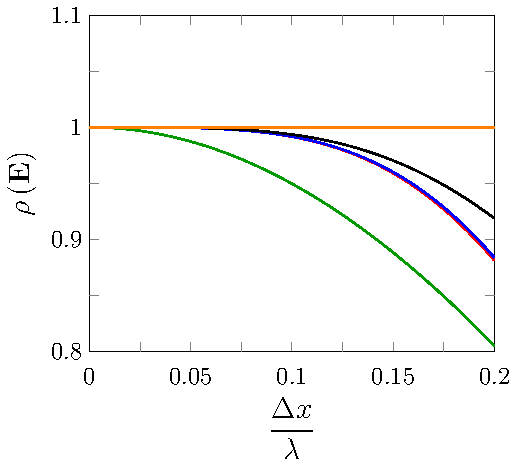
\includegraphics[width=\textwidth]{./chp4/figures/New/Stabu0.pdf}\
		\subcaption{$U=0$}
	\end{subfigure}%
	\begin{subfigure}{0.5\textwidth}
		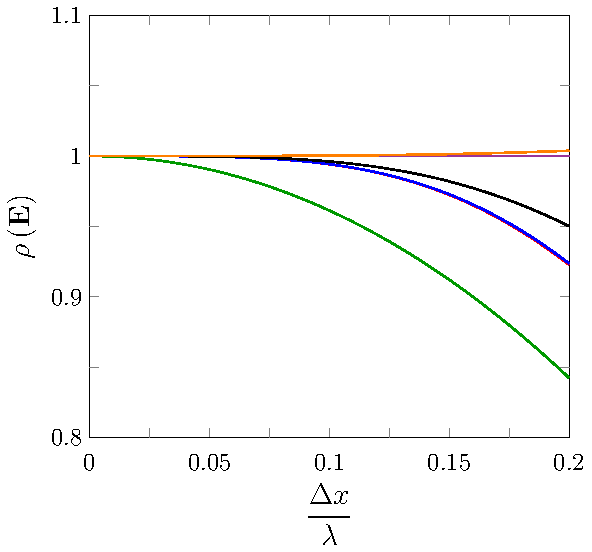
\includegraphics[width=\textwidth]{./chp4/figures/New/Stabu1.pdf}
		\subcaption{$U=1$}
	\end{subfigure}
	\caption{Spectral radius of $\matr{E}$ against $\Delta x / \lambda$ for $\text{FDVM}_1$ ({\color{green!60!black} \solidrule}), $\text{FDVM}_2$ ({\color{red} \solidrule}), $\text{FEVM}_2$ ({\color{blue} \solidrule}), $\text{FDVM}_3$ ({\solidrule}), $\mathcal{D}$ ({\color{violet!80!white} \solidrule}) and $\mathcal{W}$ ({\color{orange} \solidrule}). With $H = 1m$ and $k = {\pi}/{10}m^{-1}$.}
	\label{fig:StabShall}
\end{figure}

%The analytic value of $\rho\left(\matr{E}\right)$ is given by using \eqref{eqn:fourierfactor} to write
%\begin{equation*}
%\begin{bmatrix}
%\overline{\eta} \\ \overline{G}
%\end{bmatrix}^{n+1}_j = e^{i \omega^\pm \Delta t}\begin{bmatrix}
%\overline{\eta} \\ \overline{G}
%\end{bmatrix}^{n}_j,
%\end{equation*}
%where $\omega^\pm$ is real and given by \eqref{eqn:DispersionRelation}.
%Therefore, the analytic growth factor is
%\begin{align}
%\rho\left(\matr{E}\right) = \left| e^{i \omega^\pm \Delta t} \right| = \sqrt{\cos^2 \left(\omega^\pm \Delta t\right) + \sin^2 \left(\omega^\pm \Delta t\right)}  = 1
%\end{align}
%Thus numerical methods with $\rho\left(\matr{E}\right)$ closer to $1$ are closer to the analytic value. In this sense the two finite difference methods are best, although $\mathcal{W}$ is unstable for $U \neq 0m/s$. As expected higher-order FDVM better approximate the analytic value of the growth factor and $\lim_{\Delta x \rightarrow 0}\rho\left(\matr{E}\right) = 1$ for all numerical methods.

We observed the same results for a wide range of $k$, $H$ and $U$ values and Froude numbers. All methods except $\mathcal{W}$ were found to be stable for any combination of these variables. While $\mathcal{W}$ was only stable when $U = 0m/s$. This is different from the stability result for $\mathcal{D}$ and $\mathcal{W}$ reported by \cite{Pitt-2018-61} as that analysis assumed $U=0m/s$.


\subsection{Consistency}
%Define identity matrix?
For a numerical method to be consistent the error introduced by the method for a single time step must approach zero as the spatial and temporal resolution is increased. To demonstrate convergence, it is enough to demonstrate consistency for the eigenfunctions of the linearised Serre equations, which are the Fourier modes. Therefore, we can demonstrate consistency by investigating the evolution matrix $\matr{E}$. The error introduced for a single time step from $t^n$ to $t^{n+1}$, $\mathcal{T}^n$ is
\begin{equation}
\mathcal{T}^n =  \matr{E}\begin{bmatrix}
\overline{\eta} \\ \overline{G}
\end{bmatrix}^{n}_j -  \begin{bmatrix}
\overline{\eta} \\ \overline{G}
\end{bmatrix}^{n+1}_j.
\label{eqn:consistencyTndef}
\end{equation}
To ensure consistency we must have that $ \lim_{\Delta x,\Delta t \rightarrow 0}\left \| \mathcal{T}^n \right \|_2 = 0 $ for all $n$, where $\left \|  \cdot\right\|_2$ is the $L_2$ vector norm. Taking the $L_2$ norm of both sides of \eqref{eqn:consistencyTndef} and using \eqref{eqn:fourierfactor}  we obtain
\begin{equation*}
\left \|\mathcal{T}^n \right \|_2 = \left \|  \matr{E}\begin{bmatrix}
\overline{\eta} \\ \overline{G}
\end{bmatrix}^{n}_j -  e^{i \omega^\pm \Delta t} \begin{bmatrix}
\overline{\eta} \\ \overline{G}
\end{bmatrix}^{n}_j \right \|_2.
\end{equation*}
Using the matrix norm induced by $L_2$, the Frobenius norm $\left \|  \cdot\right\|_F$ we have that
\begin{equation*}
\left \|\mathcal{T}^n \right \|_2  \le \left \| \matr{E} -  e^{i \omega^\pm \Delta t}\matr{I} \right \|_F \left \| \begin{bmatrix}
\overline{\eta} \\ \overline{G}
\end{bmatrix}^{n}_j\right \|_2.
\end{equation*}
Since $\overline{\eta}^n_j$ and  $\overline{G}^n_j$ are finite and independent of $\Delta x$ and $\Delta t$, if $ \lim_{\Delta x,\Delta t \rightarrow 0} \left\| \matr{E} -  e^{i \omega^\pm \Delta t}\matr{I} \right\|_F = 0 $ then $ \lim_{\Delta x,\Delta t \rightarrow 0}\left \| \mathcal{T}^n \right \|_2 = 0 $ as desired.

We calculated the Taylor series of $\matr{E} -  e^{i \omega^\pm \Delta t}\matr{I}$ for all the numerical methods for all flow scenarios; subcritical, critical and supercritical flows. Since the results are the same for $\omega^+$ and $\omega^-$ we only report the results for $\omega^+$. For $\text{FEVM}_2$ the lowest order $\Delta x$ and $\Delta t$ terms of the Taylor series of $\matr{E} -  e^{i \omega^+ \Delta t}\matr{I}$ can be found in Table~\ref{tab:EerrFEVM2}. From this table it can be seen that the Taylor series of all the elements of $\matr{E} -  e^{i \omega^+ \Delta t}\matr{I}$ have a factor of $\Delta t$. So that

\begin{align*}
\left \| \matr{E} -  e^{i \omega^+ \Delta t}\matr{I} \right \|_F &=  \left \| \Delta t \left(\matr{M}_0 +  \mathcal{O}\left(\Delta t\right)\right)\right \|_F  \nonumber\\ &= |\Delta t|  \left \| \matr{M}_0 +  \mathcal{O}\left(\Delta t\right)\right \|_F
 \nonumber\\ &\le  |\Delta t| \left(\left \| \matr{M}_0 \right \|_F + \left \| \mathcal{O}\left(\Delta t\right)\right \|_F\right)
\end{align*} 
where $\matr{M}_0$ is some matrix.

From Tables~\ref{tab:EerrFEVM2} we have that $\matr{M}_0$ is independent of $\Delta t$ and finite so that as $\Delta t \rightarrow 0$ then $|\Delta t| \left(\left \| \matr{M}_0 \right \|_F + \left \| \mathcal{O}\left(\Delta t\right)\right \|_F\right)  \rightarrow 0$  and therefore  $\left \| \matr{E} -  e^{i \omega^+ \Delta t}\matr{I} \right \|_F \rightarrow 0$. Therefore, for $\text{FEVM}_2$ we have $ \lim_{\Delta x,\Delta t \rightarrow 0}\left \| \mathcal{T}^n \right \|_2 = 0 $ and so  $\text{FEVM}_2$ is consistent for Fourier mode solutions implying consistency for all solutions as desired. 

\begin{table}
	\centering
	\begin{tabular}{l c c}
		\hline 
		Element & \multicolumn{2}{c}{Lowest Order Terms of $\matr{E} - e^{i \omega^+ \Delta t} \matr{I}$ for $\text{FEVM}_2$}\T \B  \\
		  \cline{2-3}
		& $\Delta x$&$\Delta t$\T \B  \\
		\hline
		$E_{0,0} -  e^{i \omega^+ \Delta t} $& $ -\dfrac{i \left(54 + 45H^2k^2 + 10H^4k^4\right)}{120\beta^2} U k^3 \Delta t \Delta x^2$ & $\dfrac{\sqrt{3gH \beta} + 3U}{\beta} ik \Delta t$ \T \B  \\
		$E_{0,1}$& $ \dfrac{\beta - 3}{\beta^2} \dfrac{ik^3}{40} \Delta  t\Delta x^2$ &  $ - \dfrac{3}{\beta} ik\Delta t$ \T \B  \\
		$E_{1,0}$& $ -\left(gH - \dfrac{15U^2}{\beta} + \dfrac{9U^2}{\beta}\right)  \dfrac{k^3}{120}\Delta t\Delta x^2$ &  $ \left(-gH + \dfrac{3U^2}{\beta}\right)ik \Delta t$ \T \B  \\
		$E_{1,1} -  e^{i \omega^+ \Delta t}$& $ \dfrac{126 + 75H^2 k^2 + 10 H^4 k^4}{\beta^2} \dfrac{k^3}{120} i U \Delta t\Delta x^2$ & $\dfrac{\sqrt{3gH \beta} - 3U}{\beta} ik \Delta t$ \T \B  \\\hline
	\end{tabular}
	\caption{Lowest order terms of the Taylor series for the elements of $\matr{E} - e^{i \omega^+ \Delta t} \matr{I}$ for $\text{FEVM}_2$ for all values of $Fr$. Here $\beta = 3 + k^2 H^2$.}
	\label{tab:EerrFEVM2} 
\end{table}

All methods were found to be consistent using the same reasoning. Their Tables can be found in Appendix \ref{app:LinAnal}. In particular we have Tables~\ref{tab:EerrFDVM1dxerror}~and~\ref{tab:EerrFDVM1dterror} for $\text{FDVM}_1$, Table~\ref{tab:EerrFDVM2} for $\text{FDVM}_2$, Tables~\ref{tab:EerrFDVM3dxerror}~and~\ref{tab:EerrFDVM3dterror} for $\text{FDVM}_3$, Table~\ref{tab:EerrD} for $\mathcal{D}$ and Table~\ref{tab:EerrW} for $\mathcal{W}$. 

\section{Dispersion Analysis}
To study the dispersion properties of the numerical method, we must calculate the dispersion relation of the numerical method that relates the frequency $\widetilde{\omega}^\pm$ of the numerical solution to the wavenumber $k$. Making use of \eqref{eqn:fourierfactor} in \eqref{eqn:evolutionmatrix} we get
\begin{equation}\matr{E}\begin{bmatrix}
\overline{\eta} \\ \overline{G}
\end{bmatrix}^{n}_j = 
e^{i \omega^\pm \Delta t}\begin{bmatrix}
\overline{\eta} \\ \overline{G}
\end{bmatrix}^{n}_j.
\label{eqn:dispanalomeganum1}
\end{equation}
Therefore, the evolution matrix $\matr{E}$ of an exact method has the eigenvalues $e^{i \omega^+ \Delta t}$ and $e^{i \omega^- \Delta t}$ where $\omega^\pm$ are the positive and negative branches of the dispersion relation of the linearised Serre equations \eqref{eqn:DispersionRelation}. For approximate numerical methods the dispersion relation for $\widetilde{\omega}^\pm$ can be calculated by taking the eigenvalues of its evolution matrix $\lambda^\pm$ like so
\begin{equation*}
\widetilde{\omega}^\pm = \frac{1}{i \Delta t} \log\left[ \lambda^\pm\right].
\end{equation*}
By comparing $\widetilde{\omega}^\pm$ with the analytic $\omega^\pm$ given by the linearised Serre equations \eqref{eqn:DispersionRelation} we can determine the error in the dispersion relation for the numerical method. The real part of the frequency determines the speed of a wave, while the imaginary part determines the change in amplitude. For the linearised Serre equations the imaginary part of $\omega^\pm$ is zero and so the amplitude of waves are constant in time. We only present the results for the positive branch of the dispersion relation comparing $\widetilde{\omega}^+$ and $\omega^+$ as the behaviour of the negative branch is very similar. 

The relative error in the dispersion relation was plotted against $\Delta x / \lambda$ for representative values of $H$, $U$ and $k$. Where $\lambda = 2 \pi / k$ is the wavelength of the wave with wave number $k$. We used $g = 9.81m/s^2$ and chose $\Delta t = 0.5 / \left(U + \sqrt{gH}\right) \Delta x$ to satisfy the CFL condition \eqref{eqn:CFLcond}.

In Figures~\ref{fig:Dispu0Shall}~and~\ref{fig:Dispu1Shall} we present the plots for $kH = \pi / 10$ where $\sigma = kH / 2\pi =  1 / 20$ and so the water is shallow and thus the Serre equations are appropriate. We present the real and imaginary errors separately to isolate the errors in the speed and amplitude of the wave for the numerical method. The total error is also reported as a measure of the overall error in the dispersion relation of the numerical method. 

\begin{figure}
	\centering
	\begin{subfigure}{0.5\textwidth}
		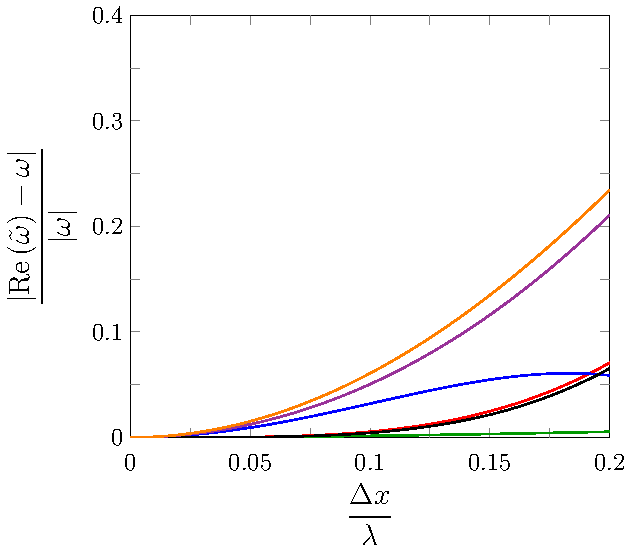
\includegraphics[width=\textwidth]{./chp4/figures/New/ReDispu0Shall.pdf}
		\subcaption{Real Part}
	\end{subfigure}%
	\begin{subfigure}{0.5\textwidth}
		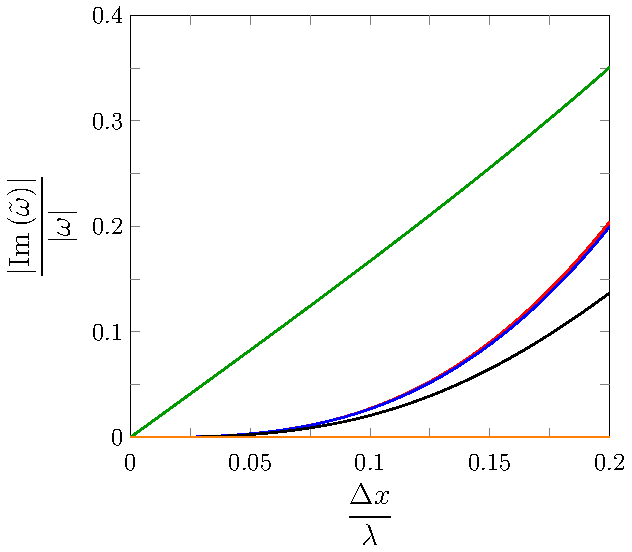
\includegraphics[width=\textwidth]{./chp4/figures/New/ImDispu0Shall.pdf}
		\subcaption{Imaginary Part}
	\end{subfigure}
	\par\bigskip
	\begin{subfigure}{0.5\textwidth}
		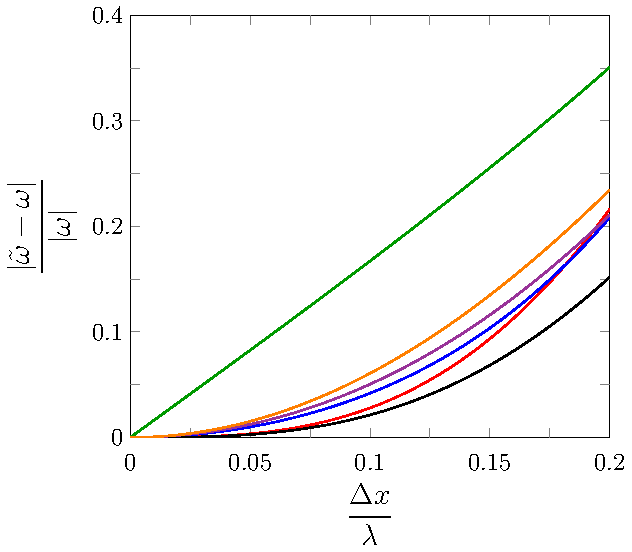
\includegraphics[width=\textwidth]{./chp4/figures/New/Dispu0Shall.pdf}
		\subcaption{Real and Imaginary Parts}
	\end{subfigure}
	\caption{Relative dispersion error against $\Delta x / \lambda$ when $H = 1m$, $k = {\pi}/{10} m^{-1}$ and $U = 0 m/s$ for $\text{FDVM}_1$ ({\color{green!60!black} \solidrule}), $\text{FDVM}_2$ ({\color{red} \solidrule}), $\text{FEVM}_2$ ({\color{blue} \solidrule}), $\text{FDVM}_3$ ({\solidrule}), $\mathcal{D}$ ({\color{violet!80!white} \solidrule}) and $\mathcal{W}$ ({\color{orange} \solidrule}).}
	\label{fig:Dispu0Shall}
\end{figure}
\begin{figure}
	\centering
	\begin{subfigure}{0.5\textwidth}
		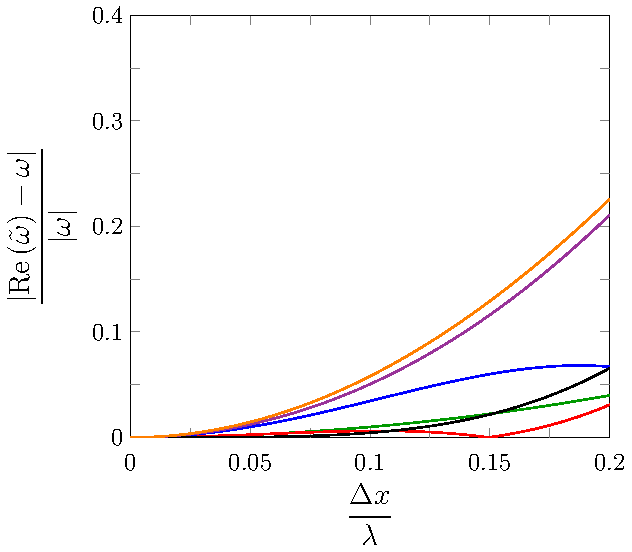
\includegraphics[width=\textwidth]{./chp4/figures/New/ReDispu1Shall.pdf}
		\subcaption{Real part}
	\end{subfigure}%
	\begin{subfigure}{0.5\textwidth}
		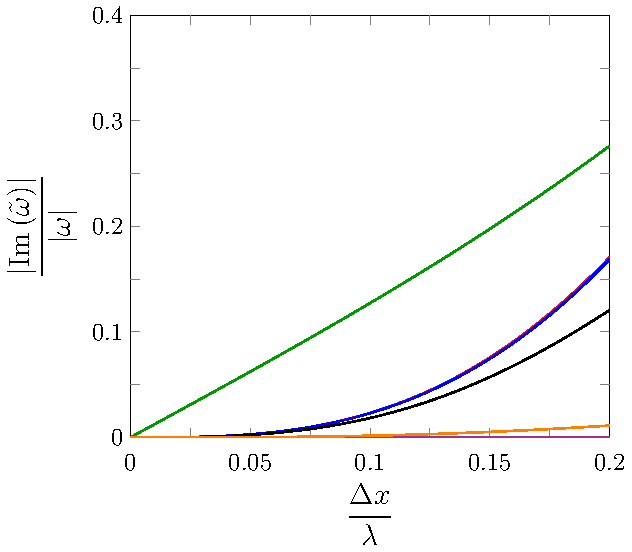
\includegraphics[width=\textwidth]{./chp4/figures/New/ImDispu1Shall.pdf}
		\subcaption{Imaginary part}
	\end{subfigure}
	\par\bigskip
	\begin{subfigure}{0.5\textwidth}
		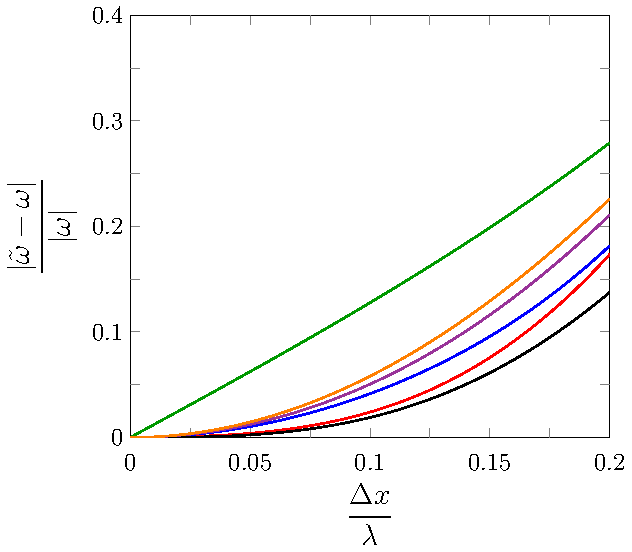
\includegraphics[width=\textwidth]{./chp4/figures/New/Dispu1Shall.pdf}
		\subcaption{Real and Imaginary Parts}
	\end{subfigure}
	\caption{Relative dispersion error against $\Delta x / \lambda$ when $H = 1m$, $k = {\pi}/{10}m^{-1}$ and $U = 1 m/s$ for $\text{FDVM}_1$ ({\color{green!60!black} \solidrule}), $\text{FDVM}_2$ ({\color{red} \solidrule}), $\text{FEVM}_2$ ({\color{blue} \solidrule}), $\text{FDVM}_3$ ({\solidrule}), $\mathcal{D}$ ({\color{violet!80!white} \solidrule}) and $\mathcal{W}$ ({\color{orange} \solidrule}).}
	\label{fig:Dispu1Shall}
\end{figure}

From Figures~\ref{fig:Dispu0Shall}~and~\ref{fig:Dispu1Shall} we can see that all methods approximate the dispersion relation of the Serre equations well with the approximation improving as $\Delta x \rightarrow 0$, as expected.

For the real part of the dispersion error all the FEVM and the FDVM outperform the two finite difference methods and therefore will better approximate the speed of waves of the linearised Serre equations. However, for the amplitude of waves the roles are reversed with the two finite difference methods either scaling the waves very little or not at all. When taking both effects into account with the total error we see that the $\text{FDVM}_1$ has the largest dispersion error followed by $\mathcal{W}$, $\mathcal{D}$, $\text{FEVM}_2$, $\text{FDVM}_2$ and finally $\text{FDVM}_3$ has the lowest dispersion error. So that the size of the total dispersion error is mainly determined by the order of accuracy of the numerical scheme. Overall the methods built around a FVM perform better than the finite difference methods of the same order. 

Furthermore, Figures~\ref{fig:Dispu0Shall}~and~\ref{fig:Dispu1Shall} demonstrate that $\text{FDVM}_2$ is superior to $\text{FEVM}_2$ not just for the complete dispersion error, but its real and imaginary parts individually as well. Therefore, $\text{FDVM}_2$ should more accurately model the speed and amplitude of waves.

We observed similar results across a wide array of $k$, $H$ and $U$ values. However, as $kH$ is increased the distinction between $\text{FDVM}_2$ and $\text{FEVM}_2$ becomes less pronounced. This can be seen in Figure~\ref{fig:Dispu0Fill} where $kH = 2.5$ and $\sigma = 5/4 \pi > 1/20$ where the water is no longer shallow.
\begin{figure}
	\centering
	\begin{subfigure}{0.5\textwidth}
		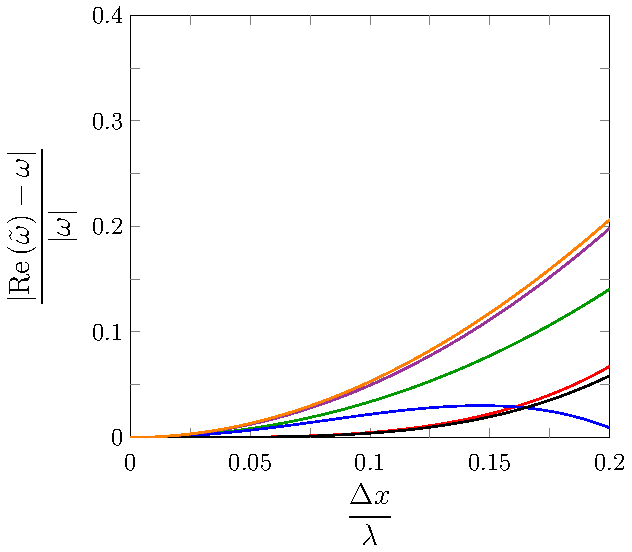
\includegraphics[width=\textwidth]{./chp4/figures/New/ReDispu0Fill.pdf}
		\subcaption{Real part}
	\end{subfigure}%
	\begin{subfigure}{0.5\textwidth}
		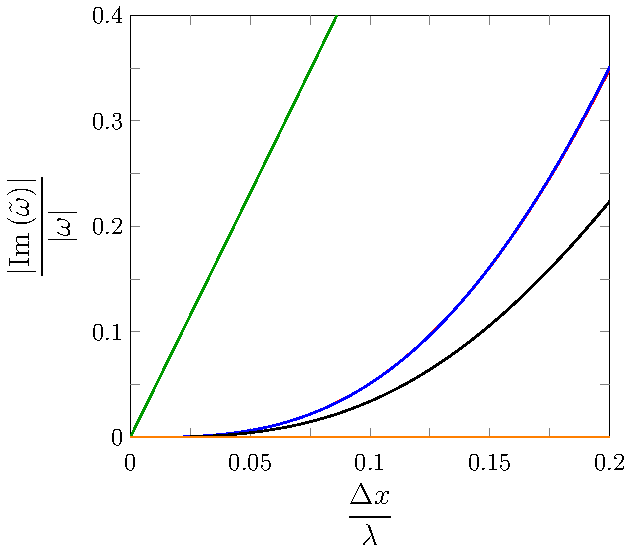
\includegraphics[width=\textwidth]{./chp4/figures/New/ImDispu0Fill.pdf}
		\subcaption{Imaginary part}
	\end{subfigure}
	\par\bigskip
	\begin{subfigure}{0.5\textwidth}
		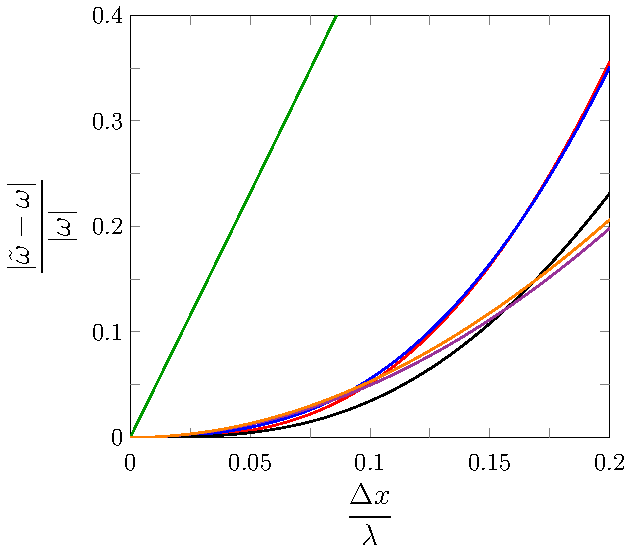
\includegraphics[width=\textwidth]{./chp4/figures/New/Dispu0Fill.pdf}
		\subcaption{Real and Imaginary Parts}
	\end{subfigure}
	\caption{Relative dispersion error against $\Delta x / \lambda$ when $H = 1m$, $k = 2.5m^{-1}$ and $U = 0m/s$ for $\text{FDVM}_1$ ({\color{green!60!black} \solidrule}), $\text{FDVM}_2$ ({\color{red} \solidrule}), $\text{FEVM}_2$ ({\color{blue} \solidrule}), $\text{FDVM}_3$ ({\solidrule}), $\mathcal{D}$ ({\color{violet!80!white} \solidrule}) and $\mathcal{W}$ ({\color{orange} \solidrule}).}
	\label{fig:Dispu0Fill}
\end{figure}

%[] put Chris reference
These $kH$ values are the same as those reported by \citet{Filippini-etal-2016-381}, and our results are similar for the real part of the dispersion error. Our FDVM and the FEVM compare favourably with the methods described and analysed by \citet{Filippini-etal-2016-381}. Furthermore, we extended their work by allowing for non-zero values of $U$, combining the spatial and temporal approximations and examining the imaginary and total error in the dispersion relation. This work also extended the dispersion analysis presented by \citet{Zoppou-etal-2017} for $\text{FDVM}_1$, $\text{FDVM}_2$ and $\text{FDVM}_3$ by including non-zero values of $U$.

Figure~\ref{fig:Dispu1Fill} demonstrates that the results of the real part of the dispersion error is slightly different if we allow for non-zero values of $U$. For example the non-zero value of $U$ significantly changes the real part of the dispersion error for $\text{FDVM}_1$ when $kH = 2.5$. Therefore, for some methods allowing for non-zero values of $U$ can have a significant impact on the conclusions drawn from the dispersion analysis. Furthermore, taking the imaginary part of the dispersion error into account is important as $\omega^\pm$ determines not only the speed of waves but also their amplitude. For instance the $\text{FDVM}_1$ performs very well for the real part of the dispersion error and poorly for the imaginary part, and so false conclusions about the accuracy of the method could be drawn from only considering the real part of the dispersion error.
\begin{figure}
	\centering
	\begin{subfigure}{0.5\textwidth}
		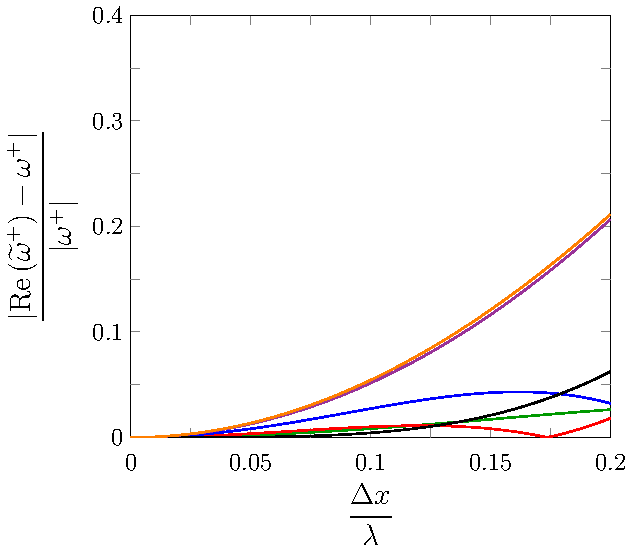
\includegraphics[width=\textwidth]{./chp4/figures/New/ReDispu1Fill.pdf}
		\subcaption{Real part}
	\end{subfigure}%
	\begin{subfigure}{0.5\textwidth}
		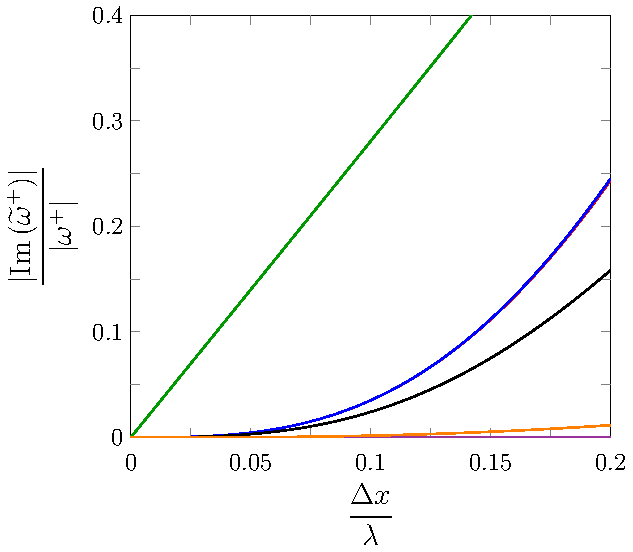
\includegraphics[width=\textwidth]{./chp4/figures/New/ImDispu1Fill.pdf}
		\subcaption{Imaginary part}
	\end{subfigure}
	\par\bigskip
	\begin{subfigure}{0.5\textwidth}
		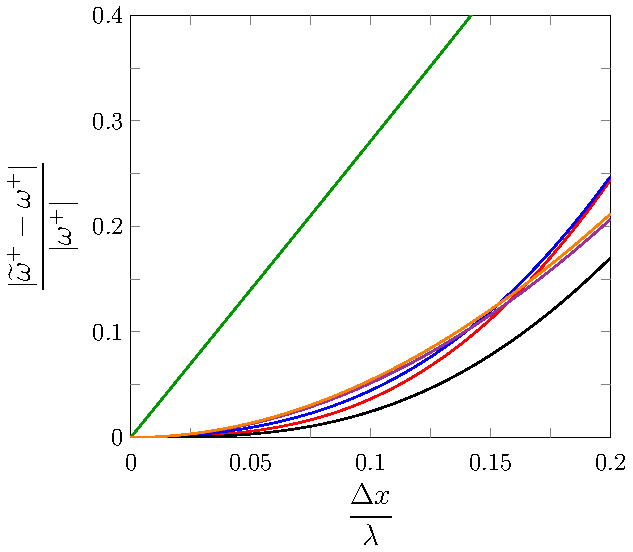
\includegraphics[width=\textwidth]{./chp4/figures/New/Dispu1Fill.pdf}
		\subcaption{Real and Imaginary Parts}
	\end{subfigure}
	\caption{Relative dispersion error against $\Delta x / \lambda$ when $H = 1m$, $k = 2.5m^{-1}$ and $U = 1m/s$ for $\text{FDVM}_1$ ({\color{green!60!black} \solidrule}), $\text{FDVM}_2$ ({\color{red} \solidrule}), $\text{FEVM}_2$ ({\color{blue} \solidrule}), $\text{FEVM}_3$ ({\solidrule}), $\mathcal{D}$ ({\color{violet!80!white} \solidrule}) and $\mathcal{W}$ ({\color{orange} \solidrule}).}
	\label{fig:Dispu1Fill}
\end{figure}

The Taylor series expansion of $\widetilde{\omega}^\pm$ was also derived for all the numerical methods. We have compiled the lowest order terms of the Taylor series for ${\widetilde{\omega}^+-\omega^+}$ in Table \ref{tab:Wfactor} when $ -1 \le Fr \le 1$ for the FDVM and FEVM. In Table \ref{tab:Wfactor} it is clear that these schemes estimated $\omega^+$ with the expected order of accuracy in both space and time. This was also the case for $\omega^-$.

We also present the lowest order terms of the Taylor series for ${\widetilde{\omega}^+-\omega^+}$ for both $ Fr < -1$ and $ Fr > 1$ in Table~\ref{tab:Wspatfactor}. We only present the errors that are different from those reported in Table~\ref{tab:Wfactor}, this was only the case for the spatial error of the first- and third--order numerical methods. From these tables it is clear that the FDVM and the FEVM retain their order of accuracy when approximating~$\omega^+$ when the flow is supercritical, this was also the case for $\omega^-$. 

Finally we present the lowest order terms of the Taylor series for ${\widetilde{\omega}^+-\omega^+}$ for the finite difference methods in Table~\ref{tab:WFDspatfactor}. These methods do not change depending on the value of the physical quantities. The two finite difference methods retain their order of accuracy in space and time when approximating~$\omega^+$.

Because all methods were demonstrated to have the expected order of accuracy in approximating $\omega^\pm$ for the linearised Serre equations this implies that for small $\Delta x$ values the order of accuracy will be the primary driver of the dispersion error, as was observed.

\begin{table}
	\centering
	\begin{tabular}{l  c  c}
	\hline
		Scheme & \multicolumn{2}{c}{Lowest Order Terms of $\widetilde{\omega}^+-\omega^+$}\T\B \\
		\cline{2-3}
		& $\Delta x$&$\Delta t$\T\B \\
		\hline
		$\text{FDVM}_1$& $-\left(2 \sqrt{gH} - \sqrt{\dfrac{3U}{\beta }}\right)  \dfrac{ik^2}{4} \Delta x$ & $\dfrac{i \left(\omega^+\right)^2}{2} \Delta t$ \T\B \\
		$\text{FDVM}_2$& $\dfrac{2\beta U -3 \sqrt{3 gH \beta}}{\beta^2}  \dfrac{k^3}{24}\Delta x ^2$ & $- \dfrac{\left(\omega^+\right)^3}{6 }  \Delta t^2$ \T\B \\
		$\text{FEVM}_2$& $\left(U   + \dfrac{\left(42 + 15 k^2H^2\right) \sqrt{3gH \beta}}{20\beta^2}  \right) \dfrac{k^3}{12 } \Delta x^2$ &  $- \dfrac{\left(\omega^+\right)^3}{6 }  \Delta t^2$ \T\B \\
		$\text{FDVM}_3$& $-\left({2\sqrt{gH} - \sqrt{3\beta}U }\right) \dfrac{ik^4}{24} \Delta x^3$ & $-\dfrac{i\left(\omega^+\right)^4}{24 } \Delta t^3$ \T\B  \\ \hline
	\end{tabular}
	\caption{Lowest order terms for Taylor series of $\widetilde{\omega}^+-\omega^+$ for all FDVM and the FEVM. With $  -1 \le Fr \le 1$ and $\beta = 3 + H^2 k^2 $. }
	\label{tab:Wfactor} 
\end{table}

\begin{table}
	\centering
	\begin{tabular}{l  c  c}
	\hline
		Scheme &\multicolumn{2}{c}{Lowest Order $\Delta x$ Term of $\widetilde{\omega}^+-\omega^+$} \T\B \\
			\cline{2-3} 
			& $Fr < - 1$&$ Fr >1$ \T\B  \\
		\hline & \\
		$\text{FDVM}_1$& $-\left(2U + \sqrt{\dfrac{3gH}{\beta}}\right)  \dfrac{ik^2}{4} \Delta x$ &  $\left(2U + \sqrt{\dfrac{3gH}{\beta}}\right)  \dfrac{ik^2}{4} \Delta x$  \T\B   \\
		$\text{FDVM}_3$& $-\left(2U + \sqrt{\dfrac{3gH}{\beta}} \right) \dfrac{ik^4}{24} \Delta x^3$ & $\left(2U + \sqrt{\dfrac{3gH}{\beta}} \right) \dfrac{ik^4}{24} \Delta x^3$  \T\B  \\
		\hline
	\end{tabular}
	\caption{Lowest order $\Delta x$ term for Taylor series of $\widetilde{\omega}^+-\omega^+$ for all FDVM for supercritical Froude numbers where different from Table \ref{tab:Wfactor}. With $\beta = 3 + H^2 k^2 $. }
	\label{tab:Wspatfactor} 
\end{table}
	
\begin{table}
	\centering
\begin{tabular}{l  c  c}
\hline
	Scheme & \multicolumn{2}{c}{Lowest Order Terms of $\widetilde{\omega}^+-\omega^+$} \T\B \\
	\cline{2-3}
	& $\Delta x$&$\Delta t$ \T\B \\
	\hline
	$\mathcal{D}$& $- \chi \Delta x^2$  &$ -\dfrac{\left(\omega^+\right)^3}{3}\Delta t^2$ \T\B  \\
	$\mathcal{W}$& $\chi\Delta x^2$  &$ \dfrac{1}{\beta^2}\Bigg( \beta U^2\left[9\sqrt{3gH \beta} + 4 \beta U\right]$ \\ & & $ + 3gH^2\left[\sqrt{3gH \beta} + 6 \beta U\right] \Bigg) \dfrac{k^3}{18 }\Delta t^2$  \T\B  \\ 
	\hline
\end{tabular}
	\caption{Lowest order terms of the Taylor series of $\widetilde{\omega}^+-\omega^+$ for $\mathcal{D}$ and $\mathcal{W}$. \\ With $\beta = 3 + H^2 k^2 $ and $\chi = \left(U + \dfrac{\left( 4 + H^2k^2\right)\sqrt{3gH\beta}}{4 \beta^2}\right)$. }
	\label{tab:WFDspatfactor} 
\end{table}
 %W x orig :  \dfrac{gH\left( 4 + H^2k^2\right)}{2 \beta \sqrt{3gH\beta}}
 
 \medskip
 
 In this chapter the convergence and dispersion properties of the numerical methods were studied using a linear analysis. The results of this analysis demonstrated the superiority of the high-order accurate FDVM and FEVM over the finite difference methods.